\documentclass[10pt, letterpaper]{article}
\usepackage[utf8]{inputenc}
\usepackage[T1]{fontenc}
\usepackage{mathptmx} % Times New Roman (Formal & Compact)
\usepackage[margin=0.75in]{geometry} % Optimized margins
\usepackage{graphicx}
\usepackage{titlesec}
\usepackage{enumitem}
\usepackage{wrapfig}
\usepackage{xcolor}
\usepackage{microtype} % Improved typography
\usepackage{babel}

% --- FORMATTING ---
\pagestyle{empty}
\setlength{\parindent}{0pt}
\setlength{\parskip}{0.5em}

% Section styling
\titleformat{\section}
    {\normalfont\large\bfseries\uppercase}
    {}{0em}{}[\titlerule]
\titlespacing*{\section}{0pt}{10pt}{5pt}

\begin{document}

% --- HEADER ---
\begin{center}
        {\Large \textbf{Empirical Musical Cartography: Quantifying Stylistic Evolution}} \\
        \vspace{0.3em}
        \textbf{Victor Gurbani} $\cdot$ Research Supplement $\cdot$ Fall 2026 Application
\end{center}

\vspace{-0.5em}

% --- BODY ---

\section*{1. Research Objective}
Musicology traditionally relies on subjective description to categorize style—classifying Chopin as ``Romantic'' or Debussy as ``Impressionist'' based on qualitative listening. This project aims to replace intuition with rigorous measurement. By building an end-to-end computational pipeline, I sought to quantify the precise harmonic, melodic, and rhythmic shifts that define the transition from the Common Practice Period (Bach, Mozart) to the late 19th/early 20th century. My goal was to determine if an algorithm could ``hear'' the difference between eras without human bias.

\section*{2. Methodology: The Computational Pipeline}
I assembled a license-safe, balanced corpus of \textbf{144 solo piano scores} (36 each by Bach, Mozart, Chopin, and Debussy) selected from the PDMX archive. To process this dataset, I engineered a Python-based toolkit utilizing the \texttt{music21} library:

\begin{itemize}[leftmargin=*, noitemsep, topsep=0pt]
        \item \textbf{Feature Extraction (36 Metrics):} The pipeline extracts interpretable descriptors across three domains:
        \begin{itemize}[leftmargin=1.5em, nosep]
                \item \textit{Harmonic:} \textbf{Chromatic Density} (measuring non-diatonic tones), \textbf{Dissonance Ratio} (passing tones vs.\ appoggiaturas), and Chord Quality distribution.
                \item \textit{Melodic:} \textbf{Pitch Entropy} (complexity of melodic line) and \textbf{Voice Independence}.
                \item \textit{Rhythmic:} \textbf{Syncopation Ratio} and \textbf{Duration Standard Deviation} (quantifying rubato/fluidity).
        \end{itemize}
        \item \textbf{Statistical Validation:} I applied one-way ANOVA and Tukey HSD post-hoc tests ($p < 0.05$) to identify which features successfully differentiate composers, correcting for False Discovery Rates (FDR) to ensure statistical rigor.
\end{itemize}

\section*{3. Key Findings}
% --- WRAPPED FIGURE (The Validation Test) ---
\begin{wrapfigure}{r}{0.5\textwidth}
        \vspace{-18pt}
        \centering
        % ENSURE THIS FILENAME MATCHES YOUR UPLOAD
        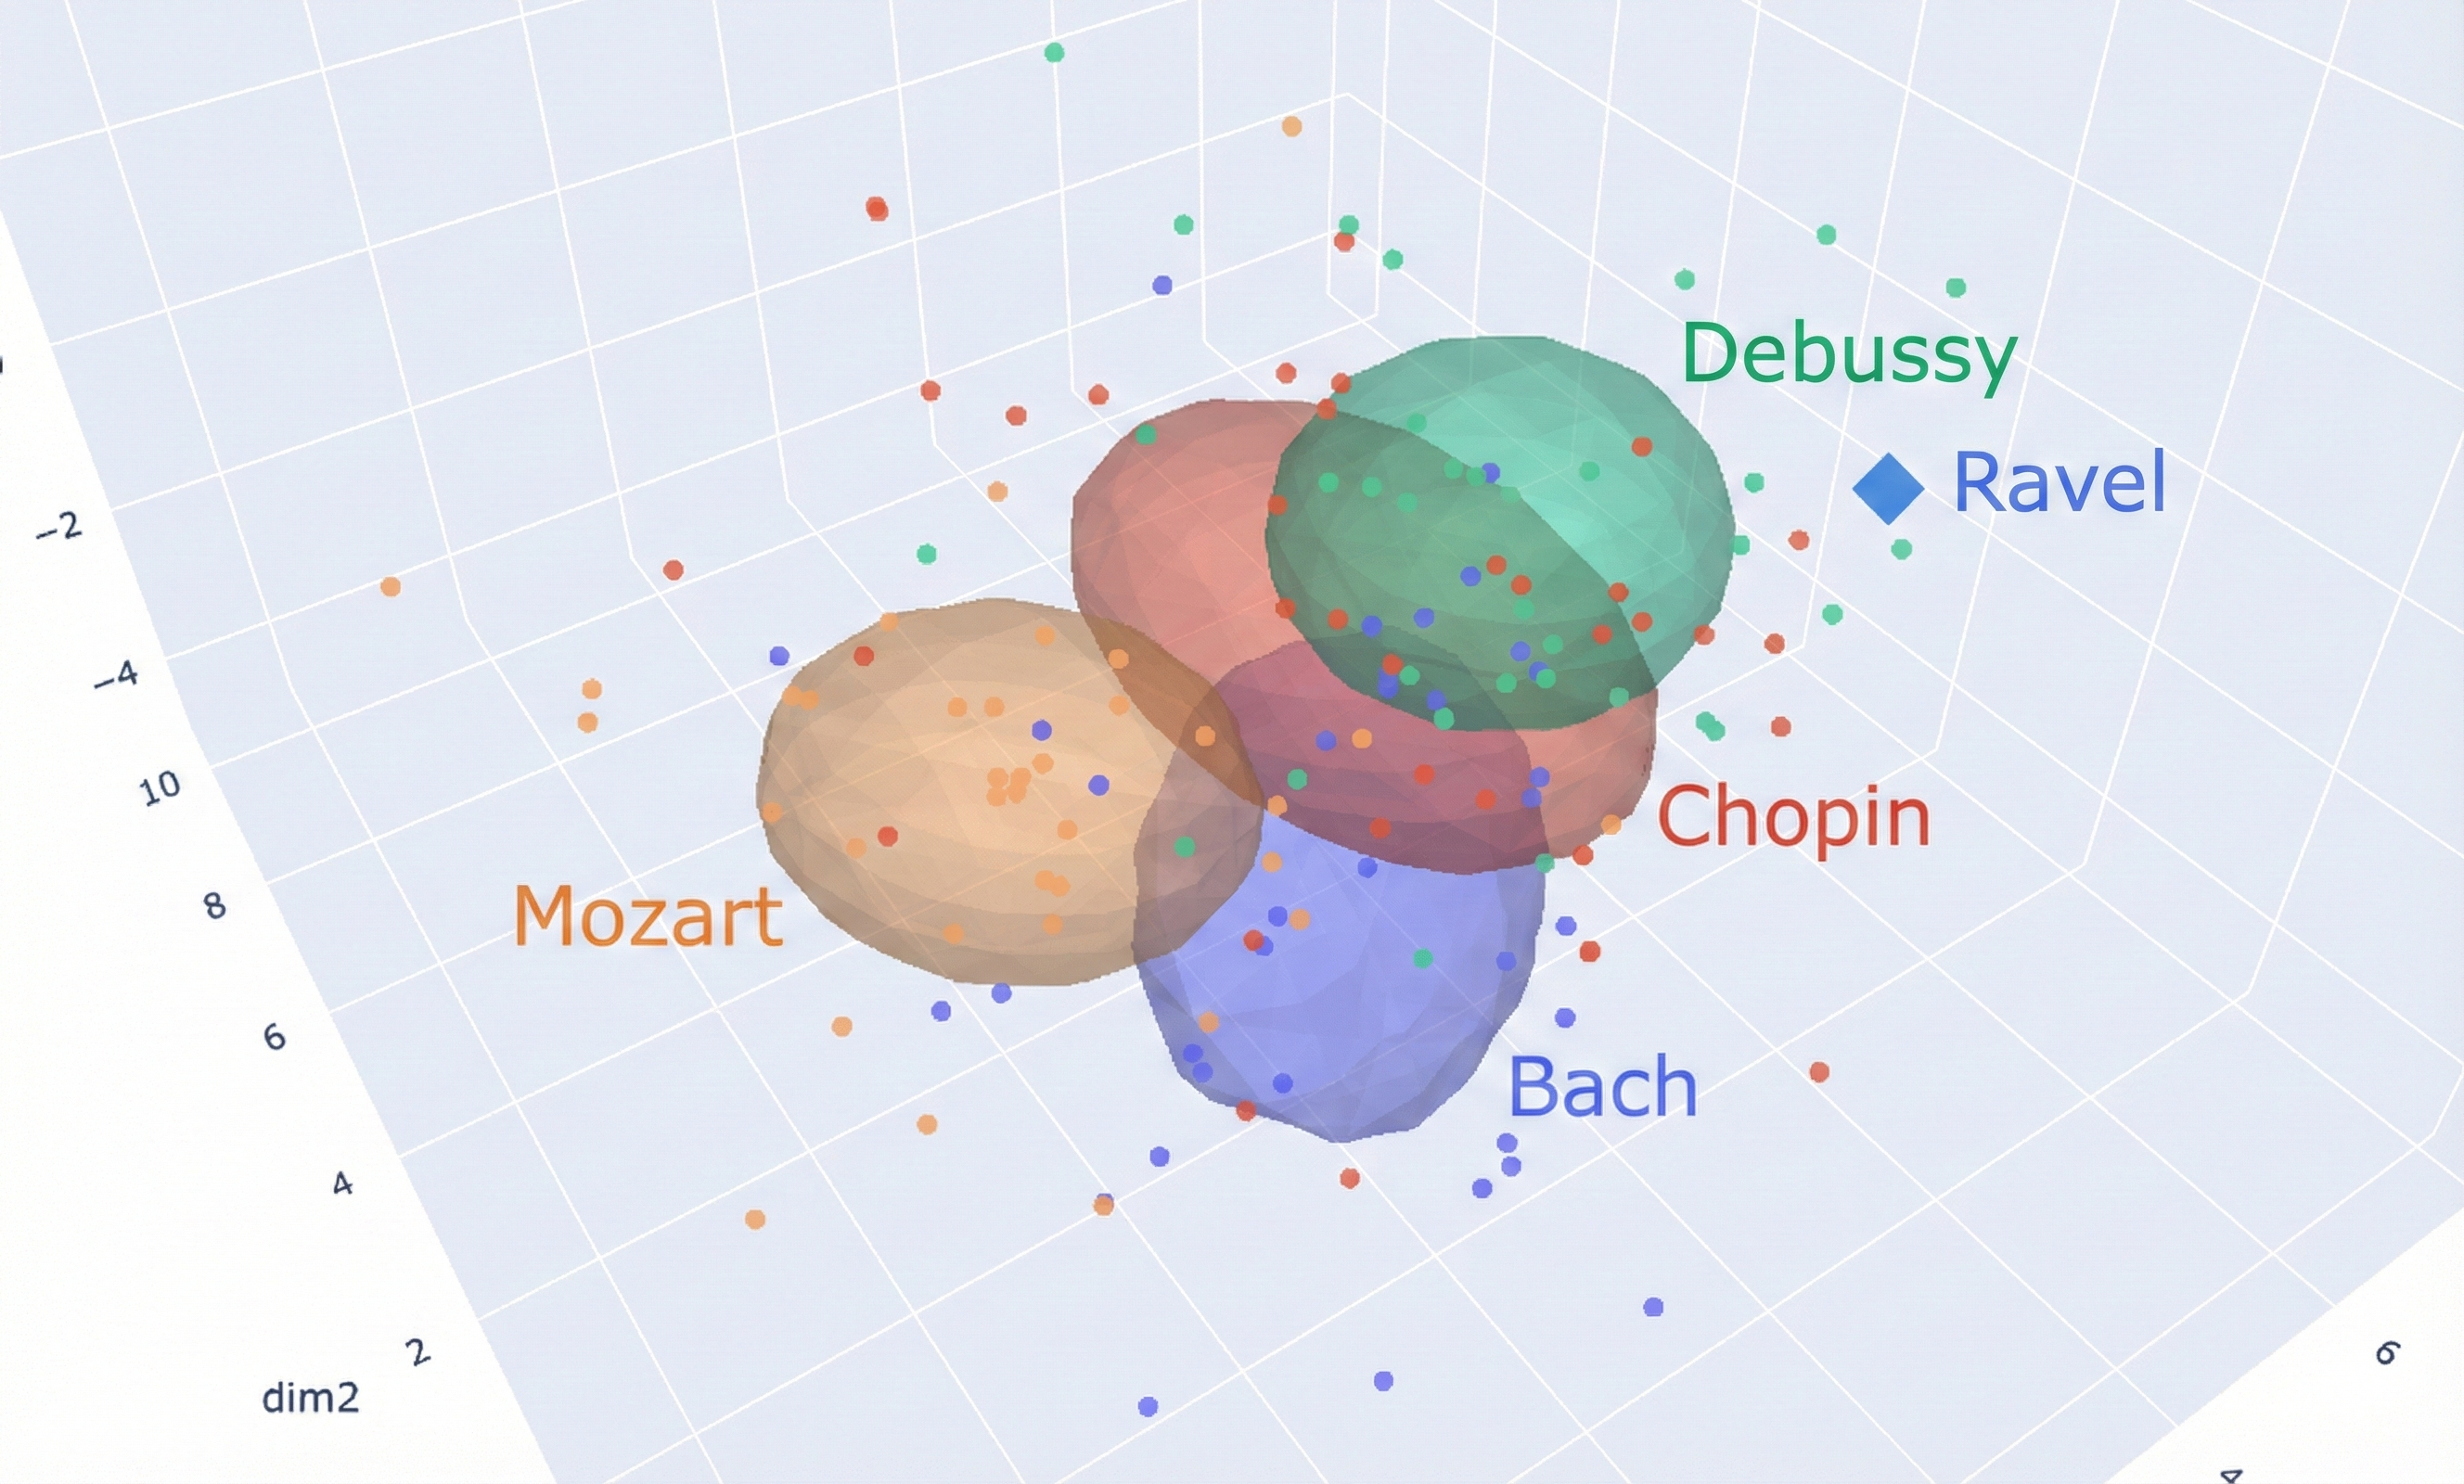
\includegraphics[width=0.48\textwidth]{ravelhighlight_cropped.png} 
        \vspace{-10pt}
        \caption{\small \textit{\textbf{Figure 1: PCA Projection of Stylistic Space.} The diamond marker ($\diamond$) represents the unseen test case: Ravel's String Quartet in F. The model correctly projects Ravel beyond the Debussy cluster, quantifying the progression into Post-Impressionism.}}
        \vspace{-10pt}
\end{wrapfigure}
Statistical analysis confirmed that \textbf{26 of the 36 metrics} are significant differentiators. The Principal Component Analysis (PCA) revealed a clear mathematical narrative, wherein the colored clouds represent the training corpus:

\begin{itemize}[leftmargin=*, noitemsep, topsep=0pt]
        \item \textbf{The ``Chopin Bridge'':} Chopin occupies a distinct transitional space. His phrasing structure (PC2) aligns with the discipline of Bach/Mozart, yet his chromatic density and rhythmic complexity (PC1/PC3) pull him toward Debussy. He acts as the mathematical link between classical clarity and impressionist color.
        \item \textbf{Differentiating Debussy:} Debussy is statistically isolated. His scores exhibit the highest dissonance rates ($p < 1.3 \times 10^{-10}$ vs.\ Bach) and rhythmic entropy, quantifying the ``blurring'' effect of Impressionism.
\end{itemize}

\section*{4. Model Validation: The ``Ravel Test''}
To test the predictive power of the model, I introduced an unseen piece outside the training corpus: \textbf{Maurice Ravel's \textit{String Quartet in F Major}}. 

As shown in \textbf{Figure 1}, the model successfully mapped Ravel into the correct stylistic region without any manual tagging. Notably, Ravel is projected \textit{further} along the primary component axis than Debussy. This mathematically confirms the musicological theory that Ravel expanded upon Impressionist textures to create even more complex, fluid structures. This result demonstrates that the 36 engineered features are not just descriptive of the past, but predictive of future stylistic evolution.

\section*{5. Significance}
This project bridges the gap between art and data science, offering a reproducible framework for ``Computational Musicology''. By treating musical scores as data, we can validate historical theories with empirical evidence, proving that the ``feeling'' of a musical era is grounded in quantifiable, mathematical structural changes.

\end{document}